%!TEX root = ../../main.tex

Como visto anteriormente, propor arquiteturas eficientes de CNNs que obtenham bom desempenho em determinada tarefa de aprendizado é considerada uma atividade difícil. Para contornar esta dificuldade, para o problema considerado neste trabalho, escolheu-se então utilizar topologias canônicas de CNNs, que obtiveram bons desempenhos reportados pela literatura, mas promovendo ajustes em seus parâmetros e hiperparâmetros com a finalidade de buscar melhorias  no desempenho para a tarefa de aprendizado aqui definida. Dentre estas arquiteturas canônicas, as selecionadas para o escopo deste trabalho encontram-se descritas a seguir:

\begin{itemize}
	\item \textbf{LeNet}. Desenvolvida por LeCun em 1989, a arquitetura LeNet foi uns dos primeiros exemplos da aplicação de CNNs, tendo sido utilizada para a detecção de dígitos manuscritos utilizando o dataset MNIST \cite{lecun}. Possui um total de 7 camadas e aproximadamente $7$ milhões de parâmetros treináveis;
	\item \textbf{AlexNet}. Em 2012, a arquitetura AlexNet foi a primeira CNN a vencer o desafio ILSVRC da ImageNet, com uma boa margem de diferença dos outros modelos submetidos à competição. Para o seu treinamento com o conjunto de dados ImageNet, foram utilizadas duas GPUs de 3 GB de memória cada, que foram capazes de armazenar o processamento de aproximadamente 62 milhões de parâmetros \cite{alexnet,khan};
	\item \textbf{MobileNet}. Constituída por um conjunto de dois hiperparâmetros, esta arquitetura possui menor latência e um tamanho menor comparada às outras arquiteturas existentes, possuindo os requisitos que facilitam a sua implementação em aplicações para dispositivos móveis e embarcados \cite{mobilenet}. No \emph{framework} \texttt{keras}, utilizado nas atividades realizadas neste trabalho, esta arquitetura possui uma profundidade de $88$ camadas, $4.253.864$ parâmetros e um tamanho de 17 MB \cite{keras};
	\item \textbf{ShuffleNet}. Esta arquitetura se destaca pela sua composição de convoluções em grupo, na qual diversas convoluções são efetuadas paralelamente tomando porções dos canais de entrada, diminuindo de maneira eficiente o custo computacional. Posteriormente, os canais de saída da convolução em grupo são mesclados aleatoriamente através do processo chamado de \emph{channel shuffle} \cite{shufflenet};
	\item \textbf{SqueezeNet}. Foi desenvolvida em 2016 através de uma parceria entre os cientistas da DeepScale, University of California, Berkeley e Stanford University. A idéia foi criar uma arquitetura com o nível de acurácia da AlexNet com $50$ vezes menos parâmetros e com um tamanho $0.5$ MB menor, permitindo uma maior eficiência no treinamento em sistemas distribuídos, menor sobrecarga na exportação de modelos através da rede e sua capacidade de ajustar-se a sistemas com pouca memória \cite{squeezenet};
	\item \textbf{VGG-16}. Esta CNN, que consiste em 16 camadas convolucionais, possui arquitetura uniforme e é comumente muito utilizada na extração de características em imagens. Possuindo mais de 138 milhões de parâmetros e uma profundidade de 23 camadas, esta arquitetura possui um tamanho total de 528 MB no módulo \texttt{applications} do \texttt{keras} \cite{vgg16, keras};
	\item \textbf{Inception}. Também chamada de GoogleNet, esta arquitetura é conhecida por ser a primeira a se desviar da forma padrão de simplesmente sequenciar camadas convolucionais e de \emph{pooling}, criando os chamados blocos \emph{Inception}. A sua versão InceptionV3 presente na biblioteca \texttt{keras} possui um total de $23.851.784$ parâmetros e um tamanho de 92 MB \cite{inception, keras}.
\end{itemize}

Em relação aos modelos adotados, considerou-se uma modificação na arquitetura geral apenas para compatibilizá-los ao problema considerado, que consiste em uma tarefa de aprendizado binária. Esta alteração diz respeito à camada de saída que consiste em apenas um neurônio com função de ativação sigmoidal, a qual retornará a probabilidade de pertencimento à cada classe na tarefa considerada.

Uma vez definidas as arquiteturas que serão utilizadas, define-se, em consequência, os parâmetros a serem adotados, que estão relacionados aos pesos destas redes, os quais serão obtidos via treinamento segundo \emph{backpropagation}. Os hiperparâmetros, por sua vez, dizem respeito  ao ajuste em nível de arquitetura das CNNs \cite{chollet}. No escopo deste trabalho, considerou-se variações nos valores dos seguintes hiperparâmetros: otimizador para o cálculo do gradiente descendente, função de ativação das camadas intermediárias e \emph{patience}, em que este último corresponde a um valor para interromper o treinamento da rede mediante \emph{early stopping} a fim de evitar \emph{overfitting}. Os valores adotados encontram-se dispostos na Tabela \ref{tab:parametros}.

\begin{table}[h!]
	\centering
	\caption{Valores dos hiperparâmetros selecionados para a elaboração dos modelos.}
	\label{tab:parametros}
	\begin{tabular}{c c C{3cm} C{3cm}}
		\toprule
		 \textbf{Épocas} & \textbf{\emph{Patience}} & \textbf{Otimizador} & \textbf{Função de ativação}  \\
		\midrule
		200 & 5, 10 e 15 & SGD, Adam e RMSprop & ReLU, ELU, SELU e Leaky ReLU \\
		\bottomrule
	\end{tabular}
\end{table}

De maneira mais detalhada, com a adoção de \emph{early stopping}, passou-se a monitorar uma métrica de desempenho durante o treinamento da rede, podendo esta ser a perda no conjunto de treinamento ou a acurácia no conjunto de validação, por exemplo. Com o uso de um valor de \emph{patience}, sempre que a métrica monitorada não melhorava durante o treinamento, decrementou-se uma unidade. O treinamento foi finalizado, então, quando este valor tornou-se igual a zero \cite{chollet}. Os valores adotados para \emph{patience}, no escopo deste trabalho, foram obtidos de maneira empírica em testes preliminares.

Um otimizador tem como objetivo aumentar o desempenho de um modelo de AM, ajustando os seus parâmetros com vistas a diminuir o erro encontrado na etapa de treinamento de tal modelo. Para o escopo deste trabalho, foram utilizados três otimizadores diferentes, sendo eles, o SGD (\emph{stochastic gradient descent}), RMSprop e o Adam (do inglês \emph{adaptive moment estimation}).

No SGD, a superfície de erro é estimada apenas com respeito a um único exemplo, tornando essa superfície dinâmica. Como resultado, descer nessa superfície melhora significativamente a habilidadede de navegar por regiões planas. O RMSprop, por sua vez, utiliza-se do valor do gradiente da função de custo e da sua raiz média quadrática para atualizar os pesos da CNN. O RMSProp tem mostrado ser um eficiente otimizador para redes neurais profundas e é a escolha principal para muitos praticantes experientes em criação de modelos de DL. E por fim, o otimizador Adam, é um algoritmo que pode ser considerado como a combinação do RMSprop com o \emph{momentum}, que possui base em estimativas adaptativas de momentos de menor ordem. É computacionalmente eficiente e demanda poucos requisitos de memória, sendo adequado para para problemas que possuem grande quantidade dados ou parâmetros \cite{buduma, rmsprop, adam}.

As funções de ativação ReLU e as suas variações \emph{Leaky} ReLU, ELU (\emph{Exponential Linear Unit}) e SELU (\emph{Scaled Exponential Linear Unit}) foram escolhidas para estarem presentes nos neurônios das camadas internas das CNNs por auxiliarem na captura de relações não-lineares. Embora a função ReLU seja amplamente adotada, optou-se também por utilizar suas variações, pois para esta pode incorrer o chamado ``\emph{dying ReLU problem}'', que acontece quando os neurônios com esta função de ativação tornam-se inativos e produzem apenas a saída zero para toda entrada \cite{reluDying}.  Desta maneira, a sua variante \emph{Leaky ReLU} mostrou ser uma boa escolha, pois possui um parâmetro adicional $\alpha$, chamado de vazamento, que faz com que o gradiente seja pequeno, mas nunca nulo. A função ELU também é uma boa alternativa à ReLU pois diminui a mudança do \emph{bias} ao pressionar a ativação média para zero. A SELU, por sua vez, possui uma auto-normalização, fazendo com que a aprendizagem seja altamente robusta e permitindo treinar redes com muitas camadas \cite{relu}. Na Figura \ref{fig:relu-variants} encontram-se os gráficos das variações da função ReLU.

\begin{figure}[h!]
	\centering
	\caption{Funções de ativação variantes da função ReLU.}\label{fig:relu-variants}
	\subfloat[\emph{Leaky} ReLu\label{subfig:lrelu}]{%
	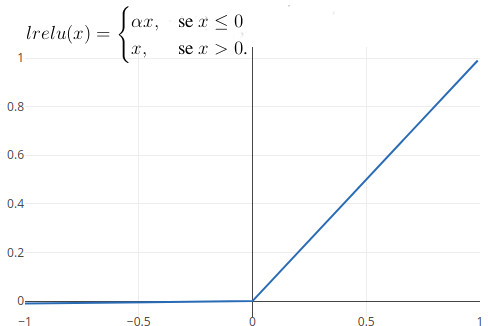
\includegraphics[width=0.5\textwidth]{imgs/lrelu}
	}
	\hfill
	\subfloat[ELU\label{subfig:elu}]{%
	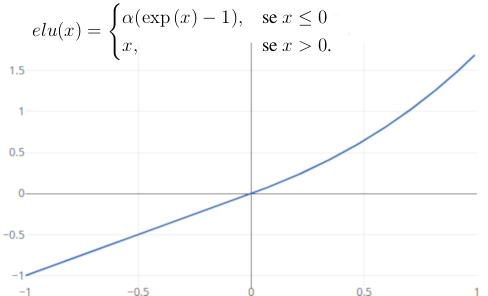
\includegraphics[width=0.5\textwidth]{imgs/elu}
	}
	\subfloat[SELU\label{subfig:selu}]{%
	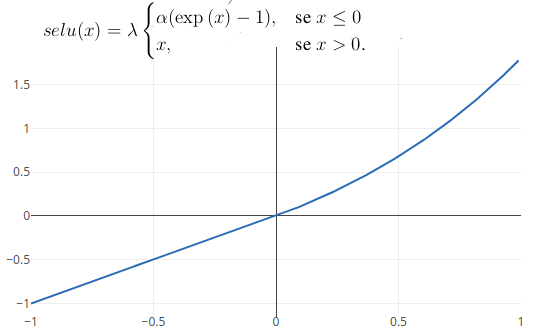
\includegraphics[width=0.5\textwidth]{imgs/selu}
	}
\end{figure}

% \begin{equation}
%     lrelu(x)=
% \begin{cases}
%     \alpha x , & \text{se } x \leq 0\\
%     x,              & \text{se } x > 0\text{.}
% \end{cases}
% \end{equation}
%
% \begin{equation}
%     elu(x)=
% \begin{cases}
%     \alpha (\exp{(x)} - 1) , & \text{se } x \leq 0\\
%     x,              & \text{se } x > 0\text{.}
% \end{cases}
% \end{equation}
%
% \begin{equation}
%     selu(x)= \lambda
% \begin{cases}
%     \alpha (\exp{(x)} - 1) , & \text{se } x \leq 0\\
%     x,              & \text{se } x > 0\text{.}
% \end{cases}
% \end{equation}

Sempre que os recursos computacionais e de tempo para o treinamento viabilizaram repetições, foram consideradas todas as variações possíveis dos hiperparâmetros descritos na Tabela \ref{tab:parametros}. Nas demais situações foram consideradas escolhas de hiperparâmetros com melhor desempenho nos cenários que já tiverem sido executados. % Ad hoc?
